% 电路与电子学III 课程笔记 —— 第1章（教材：孙立山《电路理论基础》第四版 第1章）
% 章节文件只写内容，不重复 \usepackage
\chapter{电路元件与电路基本定律}

\noindent
电路分析的任务是确定电路的行为，而电路的行为用\textbf{电路变量}（电流、电压、电荷、磁链）来表征。电路变量同时受到两种约束：
\begin{itemize}
  \item \textbf{结构约束}——由元件的连接方式决定，即基尔霍夫电流定律与基尔霍夫电压定律，与元件性质无关；
  \item \textbf{元件约束}——由元件自身的电磁特性决定，即各元件的端口方程（$u=Ri$、$q=Cu$、$\Psi=Li$ 等）。
\end{itemize}
基尔霍夫定律与元件方程联立，便得到电路方程。本章依次讨论电路变量及其参考方向、五种常用元件模型（电阻、电容、电感、独立电源、受控电源）和基尔霍夫两个定律。

\section{电流、电压与电功率}

\subsection{电流}
荷电质点的有序运动形成电流。设在时间 $\mathrm{d}t$ 内通过某截面的电荷量的代数和为 $\mathrm{d}q$，则电流定义为电荷的时间变化率
\begin{equation}
i=\frac{\mathrm{d}q}{\mathrm{d}t}
\end{equation}
其方向规定为\textbf{正电荷运动的方向}。电荷的 SI 单位为库[仑]（$\mathrm{C}$），时间的 SI 单位为秒（$\mathrm{s}$），故电流的 SI 单位为安[培]（$\mathrm{A}$），$1\,\mathrm{A}=1\,\mathrm{C}/1\,\mathrm{s}$。

一段电路中的电流有两个可能的方向。方向既可用箭头表示，也可用双下标表示：$i_{ab}$ 表示电流参考方向由 $a$ 点指向 $b$ 点，显然
\begin{equation}
i_{ab}=-i_{ba}
\end{equation}
即同一电流若参考方向取得不同，其绝对值相等而符号相反。

\begin{figure}[htbp]\centering
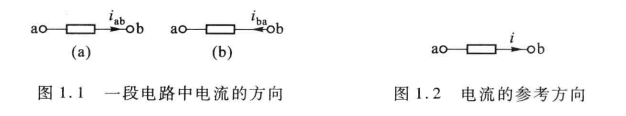
\includegraphics[width=0.72\textwidth]{1.1和1.2.png}
\end{figure}

分析复杂电路时往往难以判断电流的真实方向，而且有些电路中电流的真实方向随时间不断改变。为此，在列写电路方程时可任意假设一个方向，称为电流的\textbf{参考方向}，并用实线箭头标在图中。选定参考方向后，电流便是\textbf{代数量}：按参考方向求得的电流为正值，表明真实方向与参考方向一致；为负值则相反。电路的参考方向一经设定就不宜随意更改，否则极易导致符号混乱。

量值和方向不随时间变化的电流称为\textbf{直流}（DC），记作 $I$；随时间作周期性变化且平均值为零的电流称为\textbf{交变电流}（AC），记作 $i$ 或 $i(t)$。通常用大写字母表示直流，用小写字母表示随时间变化的量。

\subsection{电压}
单位正电荷从电路中一点移动到另一点，电场力对电荷做功。设电场力将电量为 $\mathrm{d}q$ 的正电荷由 $a$ 点移至 $b$ 点所做的功为 $\mathrm{d}W_{ab}$，则 $a$、$b$ 两点间的电压定义为
\begin{equation}
u_{ab}=\frac{\mathrm{d}W_{ab}}{\mathrm{d}q}
\end{equation}
电压的 SI 单位为伏[特]（$\mathrm{V}$）。

电压又称\textbf{电位差}。在电路中任选一点为参考点（零电位点，符号 $\perp$），某点与参考点之间的电压称为该点的\textbf{电位} $\varphi$，两点间的电压等于这两点的电位之差
\begin{equation}
u_{ab}=\varphi_a-\varphi_b
\end{equation}
电压的方向规定为从高电位指向低电位的方向，故电压有时也称为\textbf{电位降}。电压参考方向可用双下标、正负极性（$+$、$-$）或箭头三种方式表示，三者含义相同。

\corepoint{“电压”与“电位”的区别在于参考点：电位随参考点的选择而改变，两点间的电压与参考点无关。“电压降”与“电压升”只差一个符号，列 KVL 时统一按一种口径即可。}

\subsection{电动势}
电源具有将正电荷从低电位处经电源内部转移至高电位处的能力。设在 $\mathrm{d}t$ 时间内电源使正电荷 $\mathrm{d}q$ 从负极经电源内部移至正极所做的功为 $\mathrm{d}W'$，则电源的电动势定义为
\begin{equation}
e=\frac{\mathrm{d}W'}{\mathrm{d}q}
\end{equation}
即电动势的数值等于将单位正电荷从负极经电源内部移到正极时电源所做的功，其单位与电压相同。电动势的真实方向是把正电荷从低电位端移向高电位端的方向，因此\textbf{与电压的正方向刚好相反}。

\subsection{电功率}
电功率是衡量电能转换或传输速率的物理量。若在 $\mathrm{d}t$ 时间内消耗或吸收的能量为 $\mathrm{d}W$，则
\begin{equation}
p=\frac{\mathrm{d}W}{\mathrm{d}t}
\end{equation}
设某部分电路流过的电流为 $i$、端电压为 $u$，则 $\mathrm{d}t$ 内通过的电量为 $\mathrm{d}q=i\,\mathrm{d}t$，该电荷通过电路时电能所做的功 $\mathrm{d}W=u\,\mathrm{d}q=ui\,\mathrm{d}t$，于是这部分电路吸收的功率为
\begin{equation}
p=ui
\end{equation}
功率的 SI 单位为瓦[特]（$\mathrm{W}$），$1\,\mathrm{W}=1\,\mathrm{V}\times1\,\mathrm{A}$。

\textbf{关联参考方向}：同一元件上电压与电流的参考方向取成一致（电流从电压的“$+$”极流入），称为关联参考方向；否则称为非关联参考方向。功率的“吸收/发出”必须同时依据参考方向与计算结果的符号判定：

\begin{center}
\begin{tabular}{@{}lll@{}}
\toprule
参考方向 & 计算公式 & 结果为正时表示 \\
\midrule
关联 & $p=ui$ & 该部分电路\textbf{吸收}功率 \\
非关联 & $p=ui$ & 该部分电路\textbf{发出}功率 \\
\bottomrule
\end{tabular}
\end{center}

一段电路究竟是吸收还是发出功率，不会因参考方向选择不同而得出不同结论。例如某段电路 $u=-10\,\mathrm{V}$、$i=2\,\mathrm{A}$（关联），则 $p=-20\,\mathrm{W}<0$，说明它实际发出 $20\,\mathrm{W}$ 功率；若改取非关联方向，则 $u=10\,\mathrm{V}$、$p=20\,\mathrm{W}>0$，结论仍是发出 $20\,\mathrm{W}$。

功率等于能量的转换速率，在 $t_0\sim t$ 时间内电路吸收（关联参考方向）或发出（非关联参考方向）的能量为
\keyformula{W(t)=\int_{t_0}^{t}p(\xi)\,\mathrm{d}\xi=\int_{t_0}^{t}u(\xi)i(\xi)\,\mathrm{d}\xi}

实际电气设备、元器件本身都有功率限制，即\textbf{额定功率}。使用时实际功率不得超过额定值，否则（过载）会加速损耗甚至损坏设备。

\corepoint{功率计算的三步：（1）看 $u$、$i$ 是否关联；（2）按 $p=ui$ 算出代数值；（3）按上表由“参考方向＋符号”判定吸收或发出。千万不要见到负号就说“功率为负所以不消耗”。}

\section{电阻元件}
电阻元件是电阻器、白炽灯、电炉等实际器件的理想化模型，这些器件共同的特征是\textbf{消耗电能}。在电路理论中，将流过相同电流的两个端子称为一个\textbf{端口}。线性二端电阻的端口电压与电流之间遵循欧姆定律，二者成正比。在 $u$、$i$ 取关联参考方向时
\begin{equation}
u=Ri \qquad\text{或}\qquad i=Gu
\end{equation}
式中 $R$ 称为电阻[系数]，SI 单位为欧[姆]（$\Omega$），$1\,\Omega=1\,\mathrm{V}/1\,\mathrm{A}$；$G$ 称为电导[系数]，SI 单位为西[门子]（$\mathrm{S}$），$1\,\mathrm{S}=1\,\mathrm{A}/1\,\mathrm{V}$。若 $u$、$i$ 参考方向相反，两式中均应添一负号。

电阻与电导是反映同一电阻元件性能而互为倒数的两个参数
\begin{equation}
RG=1
\end{equation}

\begin{figure}[htbp]\centering
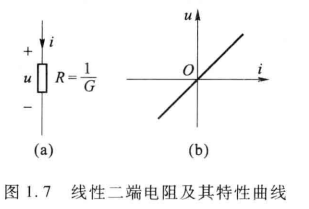
\includegraphics[width=0.5\textwidth]{1.7.png}
\end{figure}

线性电阻的端口特性在 $u-i$ 平面上是一条过原点的直线，称为电阻的电压电流关系曲线。$u$、$i$ 取关联参考方向且 $R$、$G$ 为正值时，特性曲线位于第 I、第 III 象限。

两种极端情况：
\begin{itemize}
  \item $R=0$：通过任意有限电流时电压恒为零，相当于\textbf{短路}（短路线电阻为零、电导为无穷大）；
  \item $G=0$：两端施加任意有限电压时电流恒为零，相当于\textbf{开路}（开路电导为零、电阻为无穷大）。
\end{itemize}

电阻吸收的功率为
\keyformula{p=ui=Ri^{2}=Gu^{2}}
若 $R$、$G$ 为正值，则 $p\ge 0$，这种电阻消耗电功率，属于\textbf{耗能元件}。从能量角度看，直到 $t$ 瞬间输入电阻的全部电能为
\begin{equation}
W=\int_{-\infty}^{t}p(\xi)\,\mathrm{d}\xi=\int_{-\infty}^{t}u(\xi)i(\xi)\,\mathrm{d}\xi
\end{equation}
此即物理学中的\textbf{焦耳定律}：导体或半导体电阻吸收电能并转化为热能。对于非负电阻，任一时刻该式结果非负，表明从全过程看这种元件只能吸收电能而不能发出电能——具有此种性质的元件称为\textbf{无源元件}。

若 $R<0$、$G<0$，关联参考方向下特性曲线位于第 II、第 IV 象限，电阻将输出电功率、对外提供电能，故\textbf{负电阻是一种有源元件}（可用电子线路实现，见第2章运放电路）。

从广义上讲，只要元件的端口电压、电流关系是代数方程，就属于电阻元件，其方程的一般形式为
\begin{equation}
u=u(i) \qquad\text{或}\qquad i=i(u)
\end{equation}
若 $u-i$ 关系不是过原点的直线，则称为\textbf{非线性电阻}。例如半导体二极管的电压电流关系为
\begin{equation}
i=I_0\left(\mathrm{e}^{u/U_T}-1\right)
\end{equation}
其中 $U_T$ 为热电压（常温下约 $26\,\mathrm{mV}$）。

\corepoint{判断“无源/有源”看的是元件能否对外提供能量：$R>0$ 时 $p=Ri^2\ge0$（无源），$R<0$ 时 $p<0$（有源）。这与“元件是否含电源”不是一回事。}

\section{电容元件}
电容元件是电容器的理想化模型，其电磁特性是\textbf{储存电荷与电场能量}。忽略损耗后，当极板间填充线性介质（介电常数与场强无关）时，电容储存的电荷 $q$ 与极板间电压 $u$ 成正比。若电压参考方向由正极板指向负极板，则线性电容的 $q-u$ 关系为
\begin{equation}
q=Cu
\end{equation}
式中 $C$ 为电容[系数]，单位 $\mathrm{C}/\mathrm{V}$，称为法[拉]（$\mathrm{F}$）。平行板电容器的电容为
\begin{equation}
C=\frac{\varepsilon A}{d}
\end{equation}
其中 $A$ 为每个极板的面积，$d$ 为极板间距，$\varepsilon$ 为介质的介电常数。$C$ 为常量的称为线性电容，否则为非线性电容。

\begin{figure}[htbp]\centering
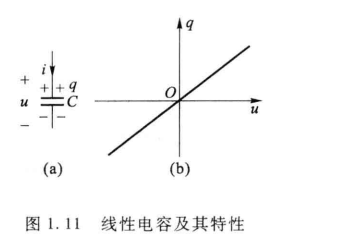
\includegraphics[width=0.55\textwidth]{1.11.png}
\end{figure}

当 $u$ 的参考方向由正极板指向负极板时，极板电荷的时间变化率就是端口电流，把 $q=Cu$ 代入得
\keyformula{i=C\frac{\mathrm{d}u}{\mathrm{d}t}}
即线性电容的端口电流与端口电压的\textbf{时间变化率}成正比。当端口施加直流电压时 $\mathrm{d}u/\mathrm{d}t=0$，端口电流为零，电容\textbf{等效成开路}。

反过来，电荷等于电流对时间的积分
\begin{equation}
q(t)=\int_{-\infty}^{t}i(\xi)\,\mathrm{d}\xi
\qquad\Longrightarrow\qquad
u(t)=\frac{1}{C}\int_{-\infty}^{t}i(\xi)\,\mathrm{d}\xi
\end{equation}
可见 $t$ 时刻电容上的电荷（电压）是此时刻以前电流充电、放电“积累”的结果，故电容具有记忆性质，属于\textbf{记忆元件}。把积分分成两段，得到常用的分段形式
\begin{equation}
u(t)=\frac{1}{C}\int_{-\infty}^{t_0}i(\xi)\,\mathrm{d}\xi+\frac{1}{C}\int_{t_0}^{t}i(\xi)\,\mathrm{d}\xi
=u(t_0)+\frac{1}{C}\int_{t_0}^{t}i(\xi)\,\mathrm{d}\xi
\end{equation}
式中 $u(t_0)$ 称为电容在 $t_0$ 时刻的\textbf{初始电压}，它代表了 $t_0$ 以前全部电流对电压的影响。

线性电容吸收的功率为 $p=ui=Cu\,\dfrac{\mathrm{d}u}{\mathrm{d}t}$。设 $t=-\infty$ 时电容尚未充电，$u(-\infty)=0$，则截止到 $t$ 时刻电容吸收的总能量为
\keyformula{W_e(t)=\frac{1}{2}Cu^{2}=\frac{q^{2}}{2C}}
这就是电容储存电场能量的计算公式。当 $u$ 的绝对值增大时 $p>0$（吸收能量），减小时 $p<0$（放出能量），故电容是\textbf{储能元件}，它不消耗能量，只是与电路交换能量。

\corepoint{电容三条推论必须记牢：（1）直流稳态下 $i=0$，电容相当于开路；（2）电容电压不能跃变（否则 $i=C\,\mathrm{d}u/\mathrm{d}t$ 将出现冲激，需无限大功率）；（3）$u$、$i$ 必须取关联参考方向，否则 $i=C\,\mathrm{d}u/\mathrm{d}t$ 前要加负号。}

\section{电感元件}
电感元件是电感线圈的理想化模型，其电磁特性是\textbf{储存磁链与磁场能量}，在周围激发磁场。若线圈的磁场存在于线性介质中，则磁链与电流成正比，称为线性电感；否则称为非线性电感。

设线性电感的磁链 $\Psi$ 与电流 $i$ 的参考方向符合右手螺旋定则，则
\begin{equation}
\Psi=Li
\end{equation}
式中 $L$ 为电感[系数]，磁链的单位为韦[伯]（$\mathrm{Wb}$），电流为安[培]时 $L$ 的 SI 单位为亨[利]（$\mathrm{H}$）。

\begin{figure}[htbp]\centering
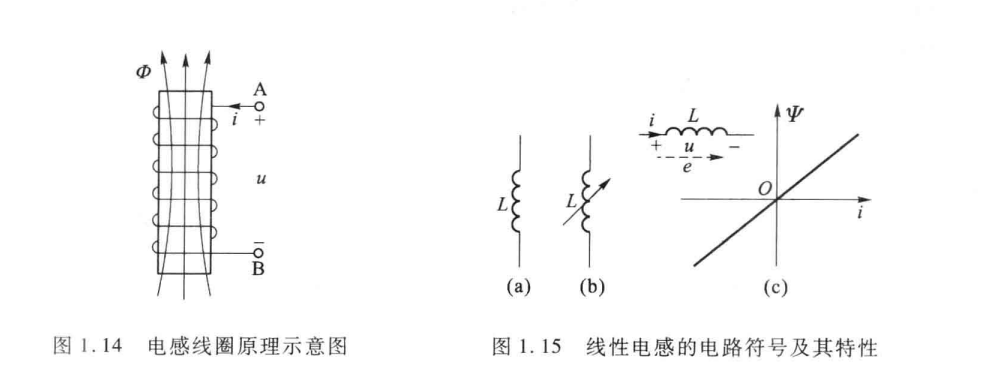
\includegraphics[width=0.5\textwidth]{1.14和1.15.png}
\end{figure}

根据电磁感应定律，磁链随时间的变化在电感中产生感应电动势 $e=-\dfrac{\mathrm{d}\Psi}{\mathrm{d}t}$。当 $u$、$e$ 与 $i$ 取关联参考方向且 $i$ 与 $\Psi$ 符合右手螺旋定则时
\begin{equation}
u=-e=-\left(-\frac{\mathrm{d}\Psi}{\mathrm{d}t}\right)=\frac{\mathrm{d}\Psi}{\mathrm{d}t}
\end{equation}
对线性电感代入 $\Psi=Li$ 得
\keyformula{u=L\frac{\mathrm{d}i}{\mathrm{d}t}}
即线性电感的端口电压与端口电流的\textbf{时间变化率}成正比。当电感中流过直流电流时 $\mathrm{d}i/\mathrm{d}t=0$，端口电压为零，电感\textbf{等效成短路}。

若由电压求磁链或电流，则需积分
\begin{equation}
\Psi(t)=\int_{-\infty}^{t}u(\xi)\,\mathrm{d}\xi=\Psi(t_0)+\int_{t_0}^{t}u(\xi)\,\mathrm{d}\xi,
\qquad
i(t)=i(t_0)+\frac{1}{L}\int_{t_0}^{t}u(\xi)\,\mathrm{d}\xi
\end{equation}
此二式表明电感中某一瞬间的磁链与电流决定于此瞬间以前的全部电压，故电感也是\textbf{记忆元件}。式中 $u$、$i$ 应为关联参考方向，否则需添负号。

线性电感吸收的功率为 $p=ui=Li\,\dfrac{\mathrm{d}i}{\mathrm{d}t}$，设 $t=-\infty$ 时 $i=0$，则截止到 $t$ 时刻电感吸收的能量为
\keyformula{W_m=\frac{1}{2}Li^{2}=\frac{\Psi^{2}}{2L}}
当电感电流的绝对值增大时 $p>0$（吸收能量并以磁场能形式储存），减小时 $p<0$（放出能量），故电感也是\textbf{储能元件}。

\corepoint{电感与电容完全对偶：$u\leftrightarrow i$、$L\leftrightarrow C$、$\Psi\leftrightarrow q$、短路 $\leftrightarrow$ 开路。记不住公式时按对偶关系推。}

三种基本无源元件的端口特性对照如下：
\begin{center}
\begin{tabular}{@{}lllll@{}}
\toprule
元件 & 特性方程 & 端口方程（关联） & 直流稳态 & 储能 \\
\midrule
电阻 & $u=Ri$ & $u=Ri$ & 有压有流 & 不储能（耗能） \\
电容 & $q=Cu$ & $i=C\dfrac{\mathrm{d}u}{\mathrm{d}t}$ & 开路 & $\frac{1}{2}Cu^{2}$ \\
电感 & $\Psi=Li$ & $u=L\dfrac{\mathrm{d}i}{\mathrm{d}t}$ & 短路 & $\frac{1}{2}Li^{2}$ \\
\bottomrule
\end{tabular}
\end{center}

\section{独立电源}
电源模型有电压源和电流源两种，它们的源电压或源电流与电路其他部分无关，故称为\textbf{独立电源}。

\subsection{电压源}
电压源能够提供确定的源电压 $u_s$。所谓“确定”是指 $u_s$ 与流过电压源的电流无关，而电压源的电流由与其相连的外电路决定。$u_s$ 为常量时称为直流电压源（恒定电压源），记作 $u_s=U_s$；也可以是时变量。源电压的方向从“$+$”极到“$-$”极。其端口特性为
\begin{equation}
u=u_s
\end{equation}
式中不含电流 $i$，表明源电压不受电流制约。$u_s$ 为常量时特性曲线是 $u-i$ 平面上平行于电流坐标轴的直线。当 $u_s=0$（电压源置零）时，其作用相当于\textbf{短路}。

按 $u$、$i$ 取非关联参考方向（电源内部从“$-$”到“$+$”），电压源发出的功率为
\begin{equation}
p=u_si
\end{equation}
$p>0$ 表示电源输出功率（供电），$p<0$ 表示电源吸收功率（充电）。

\subsection{电流源}
电流源能够提供确定的源电流 $i_s$，它与电流源端口电压无关，而端口电压由外电路决定。$i_s$ 为常量时记作 $i_s=I_s$。其端口特性为
\begin{equation}
i=i_s
\end{equation}
式中不含电压 $u$，特性曲线是平行于电压坐标轴的直线。当 $i_s=0$（电流源置零）时，其作用相当于\textbf{开路}。电流源输出的功率为 $p=ui_s$。

内阻 $R_i=0$ 的电压源与内导 $G_i=0$（内阻无穷大）的电流源分别称为\textbf{理想电压源}与\textbf{理想电流源}。由于零不能取倒数，理想电压源与理想电流源之间不能相互等效，是相互独立的两种电源模型（实际电源的两种模型及其等效变换见 §2.2）。

\corepoint{电压源置零 = 短路，电流源置零 = 开路，这两句是后面用叠加定理、戴维宁定理求等效电阻的基础，务必分清。另外“电压源不允许短路、电流源不允许开路”是理想电源的使用限制。}

\section{受控电源}
在电路模型中还要用到另一类电源，它们的源电压或源电流受电路中另一处的电压或电流控制，称为\textbf{受控电源}（非独立电源）。受控源是用来表示一条支路与另一条支路之间存在\textbf{耦合}关系的电路模型。本书只讨论线性受控源，即源电压（流）与控制电压（流）成正比。

控制量可以是电压或电流，被控制量也可以是电压或电流，故共有四种受控源：

\begin{center}
\begin{tabular}{@{}llll@{}}
\toprule
类型 & 简称 & 端口方程 & 控制系数量纲 \\
\midrule
电压控制电压源 & VCVS & $u_s=\mu u_c$ & 无量纲 \\
电流控制电压源 & CCVS & $u_s=r\,i_c$ & 电阻（$\Omega$） \\
电压控制电流源 & VCCS & $i_s=g\,u_c$ & 电导（$\mathrm{S}$） \\
电流控制电流源 & CCCS & $i_s=\beta\,i_c$ & 无量纲 \\
\bottomrule
\end{tabular}
\end{center}

式中带脚注 $s$ 的变量表示源，带脚注 $c$ 的变量表示控制量，$\mu$、$r$、$g$、$\beta$ 均为常量。

\begin{figure}[htbp]\centering
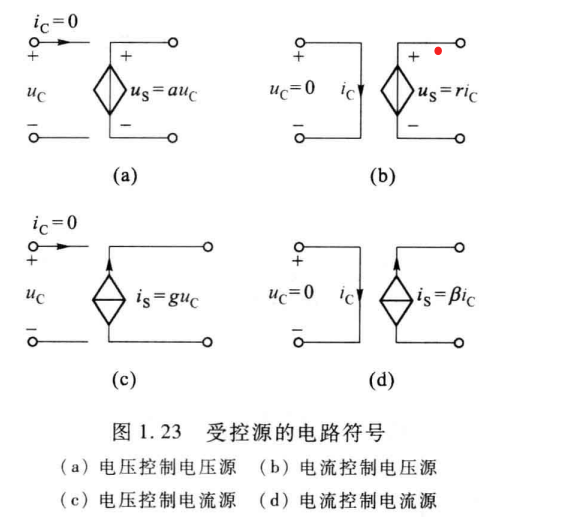
\includegraphics[width=0.72\textwidth]{1.23.png}
\end{figure}

受控源有两个端口，属\textbf{二端口元件}。由于它的控制量或是开路电压、或是短路电流，一般在电路图上不必专门画出控制端口，只需在菱形符号旁注明控制关系，并在电路中明确标注控制量即可。

受控源是电子线路中常用的电路模型。例如共射极接法的晶体管，其集电极电流 $i_c$ 与基极电流 $i_b$ 的关系为 $i_c=\beta i_b$，故其模型包含一个电流控制电流源。

\corepoint{受控源与独立源同属有源元件，但受控源本身不能提供能量：晶体管模型里受控源的能量归根结底来自外加直流电源。列写电路方程时，受控源先按独立源处理，再用待求量表示其控制量以消去中间变量（见第2章）。}

\section{基尔霍夫定律}
1847 年基尔霍夫建立了电路结构对电流、电压的约束关系，分别称为基尔霍夫电流定律（KCL）与基尔霍夫电压定律（KVL），统称基尔霍夫定律。

\subsection{电路结构}
电路结构用支路、节点、回路、网孔等术语描述。本书将每个二端元件称为一条\textbf{支路}；若干支路的连接点称为\textbf{节点}，其中两个支路的连接点称为\textbf{简单节点}。在节点 $a$ 到节点 $b$ 之间，由 $m$ 条不同支路和 $m-1$ 个不同节点（不含 $a$、$b$）依次连接成的一条通路称为 $a$ 到 $b$ 的\textbf{路径}，$a$、$b$ 分别称为始端节点和终端节点。

闭合的路径称为\textbf{回路}，回路有顺时针、逆时针两个方向。将电路画在平面上，若除节点外各支路都不相交，则称为\textbf{平面电路}，否则称为非平面电路。平面电路的单孔回路（内部或外部不包含任何支路）称为\textbf{网孔}，它是最简单的回路；内部不含支路的网孔称为内网孔，外部不含支路的称为外网孔，若无特别说明网孔均指内网孔。

一条支路若不管电流为何有限值电压恒等于零，则称为\textbf{短路}；若不管电压为何有限值电流恒等于零，则称为\textbf{开路}（断路）。

\begin{figure}[htbp]\centering
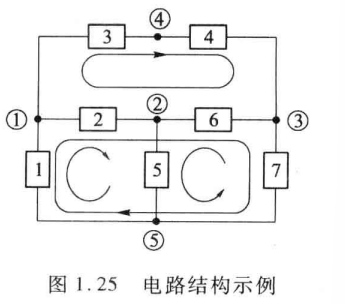
\includegraphics[width=0.62\textwidth]{1.25.png}
\end{figure}

\subsection{基尔霍夫电流定律}
\textbf{KCL}：在集中参数电路中，任一时刻流出（或流入）任一节点的支路电流的代数和等于零，即
\keyformula{\sum_{k=1}^{b} i_k=0}
通常规定：$i_k$ 的参考方向为\textbf{流出}节点时前面取“$+$”号，流入节点时取“$-$”号。该式称为节点的 KCL 方程，它反映了与任一节点相连的所有支路电流所满足的约束。

KCL 还可推广用于闭合边界，称为\textbf{广义基尔霍夫电流定律}：在集中参数电路中，任一时刻流出（或流入）任一闭合边界 $S$ 的支路电流的代数和等于零
\begin{equation}
\sum_{\text{流出}S} i_k=0
\end{equation}
由于流入任一节点的电流代数和为零，把闭合边界内各节点的 KCL 方程相加即得广义 KCL。由此还可得等价表述：任一时刻，流出任一节点（或闭合边界）电流的代数和等于流入该节点电流的代数和
\begin{equation}
\sum i_{\text{出}}=\sum i_{\text{入}}
\end{equation}

独立性：含有 $n$ 个节点的电路中，任意 $n-1$ 个节点的 KCL 方程是一组独立方程，这些节点称为\textbf{独立节点}；第 $n$ 个节点的 KCL 方程必是其余 $n-1$ 个方程的代数和。至于选哪 $n-1$ 个节点作独立节点则是任意的。

\subsection{基尔霍夫电压定律}
\textbf{KVL}：在集中参数电路中，任一时刻沿任一回路各支路电压的代数和等于零，即
\keyformula{\sum_{k=1}^{b} u_k=0}
通常规定：$u_k$ 的参考方向与回路方向\textbf{相同}时前面取“$+$”号，否则取“$-$”号。该式称为回路的 KVL 方程，它是任一回路所包含的支路电压必须满足的约束。

推广形式一：沿任一回路，各支路\textbf{电压降}的代数和等于\textbf{电压升}的代数和
\begin{equation}
\sum u_{\text{降}}=\sum u_{\text{升}}
\end{equation}
教材中常见写法为 $\sum u=0$（绕行一周电压降之和为零）与 $\sum u_{\text{升}}=0$ 两种口径，二者只差一个符号。

推广形式二：集中参数电路中，\textbf{任意两点之间的电压具有确定值，与计算路径无关}（即电压与路径无关，只与两端点有关）。这一性质是把“两点间电压”写成“沿某条路径的电压降之和”的依据。

设电路有 $b$ 条支路、$n$ 个节点，则独立 KVL 方程的个数（独立回路数）为
\begin{equation}
m=b-(n-1)
\end{equation}
对平面电路的全部内网孔列出的 KVL 方程必是一组独立方程；反之，任一网孔的 KVL 方程不能表示为其余网孔 KVL 方程的线性组合。取网孔只是获得独立 KVL 方程的\textbf{充分条件}而非必要条件，例如“两个网孔＋一个非网孔回路”也可以是独立组，但独立方程的数目总是一样的。

\corepoint{基尔霍夫定律只与电路结构有关，\textbf{与元件性质无关}：无论元件是线性还是非线性、含源还是无源、时变还是非时变，KCL、KVL 都成立；KVL 还可用于含“假想支路”（断开处）的假想回路。这正是它被称为“结构约束”的原因。}

\subsection{两类约束与列方程的思路}
列写电路方程时，KCL 约束的是与节点相连的支路电流，KVL 约束的是回路所包含的支路电压，二者提供的独立方程数为 $(n-1)+[b-(n-1)]=b$；再与 $b$ 个支路的元件方程联立，即可解出 $b$ 个支路电流（或电压）。这一思路在下一章发展为支路电流法、回路电流法和节点电压法。

\begin{center}
\begin{tabular}{@{}lll@{}}
\toprule
约束类型 & 依据 & 独立方程数 \\
\midrule
结构约束（KCL） & 节点电流代数和为零 & $n-1$ \\
结构约束（KVL） & 回路电压代数和为零 & $b-(n-1)$ \\
元件约束 & 各元件端口方程 & $b$ \\
\bottomrule
\end{tabular}
\end{center}

\endinput
